\fancychapter{Introduction}
\cleardoublepage
\label{chapter:1}

\section{Context}
% What is language and speech
The faculty of expressing or describing thoughts, feelings and needs by using language is a fundamental ability in our daily lives. As per by the Oxford dictionary,  \textit{language is defined as the system of communication in speech and writing that is used by people of a particular country or area}. Consequently, language can be conceptualised as a intricate and rule-governed system that empowers individuals to convey abstract concepts, share experiences, and take part in nuanced forms of communication. Effective communication through language begins with the conceptualization of the message to be transmitted (\textit{conceptualisation}), followed by the selection of appropriate lexical items and subsequent grammatical encoding, culminating by their meaningful organisation (\textit{formulation}). Subsequently, the linguistic representation is transformed into sound through the transmission of this representation from the brain to the muscles of the complex speech system including lips, larynx, glottis, lungs, jaw and tongue (\textit{articulation}) \cite{levelt1993speaking}. Unlike language, which encompasses both spoken and written forms, speech specifically refers to the spoken manifestation of language.


% Children speech and language acquisition
This capability to speak and comprehend language is not inherently present but rather develops gradually over time with experience. Babies  instinctively engage in pre-linguistic communication, using gestures, facial expressions, and vocalisations to articulate their basic needs. As language acquisition progresses, children transition to the babbling stage, experimenting with sound patterns. Eventually, speech emerges, marking a crucial milestone in communication development, and typically, children reach specific language milestones at particular ages. For example, around 12 to 18 months, a child usually utters their first words and starts imitating sounds. By the age of 4 to 5, children tend to formulate sentences and grasp more intricate concepts. Regarding speech sounds, younger children, approximately 1 year old, can produce basic speech sounds like \textit{/p/}, \textit{/b/}, \textit{/m/} while older children, around 5 years old, can articulate more complex sounds such as \textit{/r/} and \textit{/th/}. This developmental stage is referred as language acquisition, and it plays a crucial role in a child's overall development. Indeed, our daily dependence on social and communication skills endures throughout our entire lives. Consequently, it is imperative for children to develop the capacity to interact effectively with others to achieve seamless integration into society across all aspects of their lives.

% But pathology exists, need for therapy/assessment
Regrettably, a subset of children experience speech disorders stemming from congenital conditions such as cleft palate, cerebral palsy, and prelingual deafness. Alternatively, certain individuals may acquire speech-related issues during childhood, encompassing cognitive developmental delays, breathing-feeding-swallowing disorders and traumatic brain injuries. Notably, in 2012, empirical data \cite{black2015communication} highlighted that 7.7\% of children aged 3 to 17 in the United States exhibited communication disorders, with 5.0\% of this cohort specifically presenting speech-related problems.

Furthermore, findings \cite{langbecker2020long} suggests that individuals afflicted with childhood speech disorders may confront an increased prevalence of mental health challenges, diminished social well-being, and reduced academic accomplishments in comparison to their peers. This highlights the complex nature of speech disorders in children,  the consequences of which extend into adolescence and adulthood. Hence,  early identification and intervention play a pivotal role in mitigating the enduring effects on these children's social interactions, society integration, communication skills, educational progress, and overall well-being.

% Speech therapy
Pediatric Speech and Language Pathologists (SLPs) play a crucial role in providing therapy to help children overcome the effects of speech disorders and offer early diagnosis. The therapy typically includes exercises and assessments, which can be based on perceptual speech evaluations or standardised tests. To effectively engage children, these activities are often presented as games, taking into consideration the inherently limited attention span of children. Notably, SLPs frequently maintain long-term follow-ups with their patients, allowing them to monitor the evolution of speech quality over time and tailor exercises to the specific needs of each child. The adoption of this individualised therapeutic approach is essential for helping children achieve improved speech and communication skills.

% Problems with speech therapy (hospital, stress, ...)
However, a prominent challenge arises concerning the accessibility and availability of speech therapy services. Numerous children, particularly those residing in underserved or remote areas, encounter obstacles in accessing speech therapy resources. Additionally, the hospital environment introduces an additional layer of stress for children. While clinically necessary, the setting may inadvertently contribute to heightened anxiety and discomfort, as children may perceive it as intimidating. Furthermore, the logistical challenges associated with frequent hospital visits impose a substantial financial and time burden on families.

Another obstacle pertains to the continuity and consistency of therapy. Children may experience interruptions in their therapeutic journey due to factors such as financial constraints, scheduling conflicts, or alterations in healthcare coverage. These disruptions have the potential to impede progress and undermine the effectiveness of the therapy. Lastly, it is imperative to acknowledge that, despite professional training, inter-expert variability in perceptual assessments may persist, resulting in disparate diagnostic conclusions. To address these challenges, adopting a hybrid approach that combines in-person therapy with technology holds potential benefits \cite{hilty2015new,barnett2011utilizing}. Teletherapy, for instance, has emerged as a promising avenue to bridge geographical gaps and deliver therapy services remotely \cite{hughes2019increasing}.

\begin{figure}
    \centering
    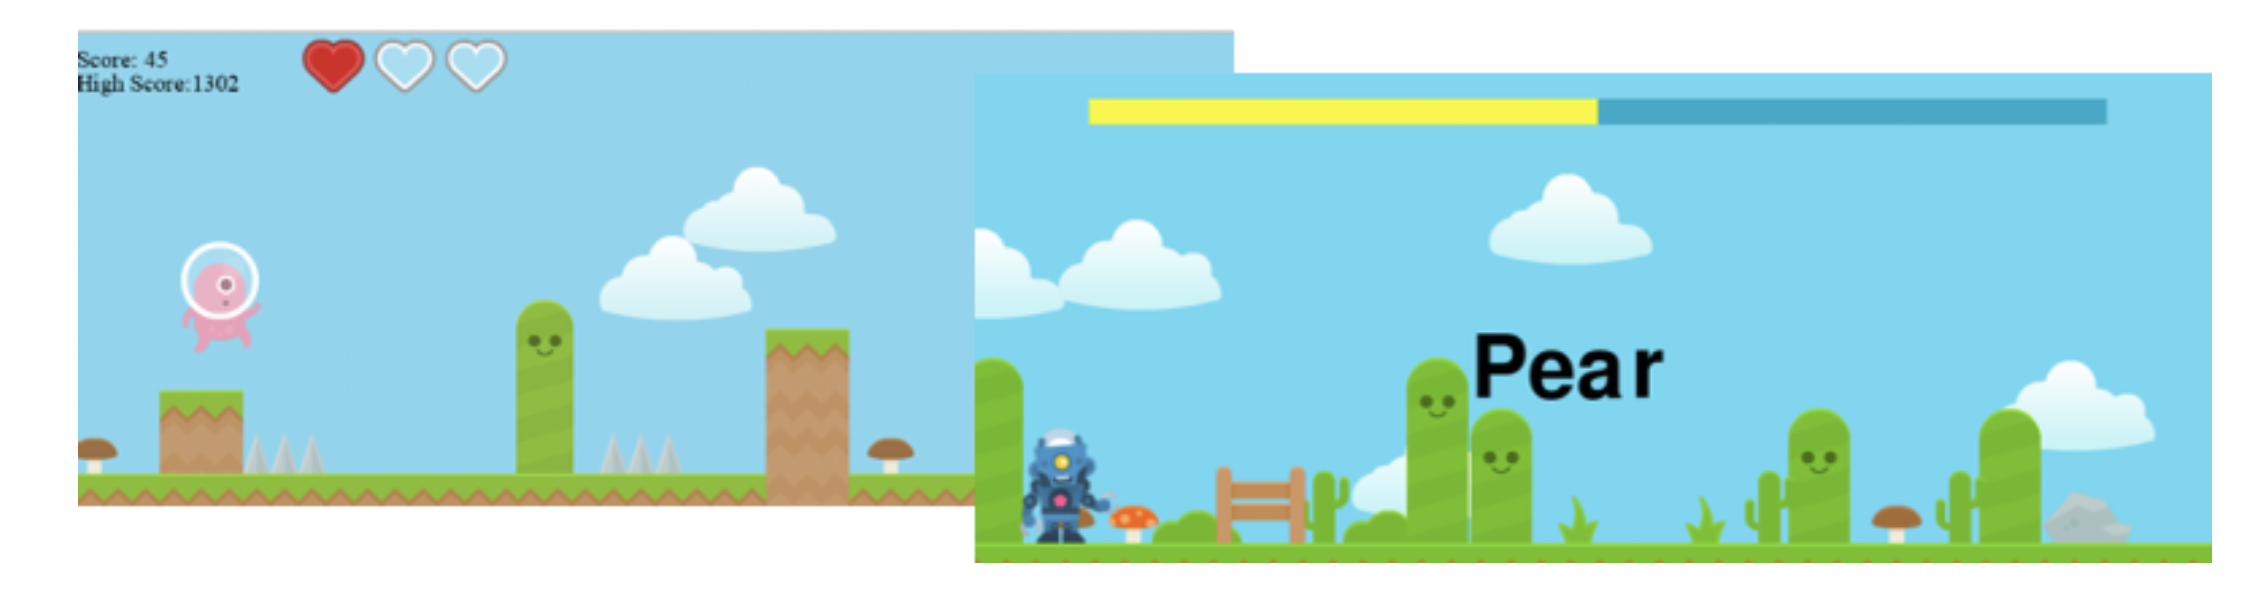
\includegraphics[width=1\textwidth]{imgs/exampleSLT.png}
    \caption{Illustrated herein are some examples of children's Speech and Language Technology applications that were developed during the course of this thesis. On the left is a running platformer game, where the user's voice controls the character. Pitch dictates running and jumping actions, while energy modulates the velocity of these actions. On the right, a reading task game is depicted, wherein a robot instructs the user to read designated words.}
    \label{fig:exSLT}

\end{figure}

% SLT could be the beginning of the answer and is already used in real life
In this context, Speech and Language Technologies (SLT) have emerged as highly pertinent within the domain of speech therapy \cite{mendoza2022added}. These technologies encompass a spectrum of computational tools designed to analyse, understand and provide objective and precise automated assessments. Another benefit lies in their potential integration into gamification frameworks, thereby augmenting children's involvement during therapy \cite{brewer2013using}. Moreover, the ability to record speech utter by the patient during a session using SLT enables post-session thorough analysis and long-term monitoring by the therapist. Due to the aforementioned reasons, the development of such tools has gained considerable attention, empowering patients to engage in exercises beyond therapy sessions, notably in a home setting. Several SLT examples developed within the scope of this thesis are illustrated in Figure \ref{fig:exSLT}.

\section{Problem statement}
% Technologies are more and more present
Recent years have seen an increased integration of SLT into various aspects of our daily lives, impacting a wide range of environments, including homes, transportation, education, and even the military. Noteworthy examples encompass voice assistants, hands-free computing, healthcare systems, automatic helplines, and speech-to-speech translation services. The performances progress in these applications was made possible through the use of machine learning techniques, espacially deep learning approaches, the increasing computational capacities of our devices, and the ever-growing volume of data available to train and improve these systems.

% Children are a good target audience for SLT
Children represent a promising target audience for SLT due to the inherent complexities of conventional computer interfaces, which pose challenges for them, limiting their capacity to fully benefit from digital platforms. Children commonly face difficulties to manipulate mouse and keyboard inputs. Additionally, the abstract nature of traditional man-machine interfaces can impede the understanding necessary for effective interaction. In this context, speech-based systems emerge as a promising alternative, offering a more natural and accessible means for children to interact with technology. Through the use of speech recognition technologies, these speech systems mitigate the barriers associated with conventional interfaces, providing a fluid and intuitive interaction paradigm that aligns more closely with the developmental stages and cognitive abilities of young users.

% Automatic tools for speech therapy
As previously mentioned, SLTs are gradually making their way into the field of atypical speech, particularly for children. While these automatic tools are currently in their early stages and have limitations, there is indeed a rising interest in implementing atypical speech and language therapy cutting-edge systems with a focus on assisting SLPs. In this context, systems capable of automatically recognising speech content, assessing pronunciation quality and detecting speech pathologies could be highly valuable in supporting pediatric SLPs and patients.

All of these objectives require the implementation of a robust automatic speech recognition (ASR) system specifically tailored for healthy children, serving as a foundational model. Nevertheless, while speech recognition technologies have made substantial advancements, leading to increased accuracy, the performance of ASR systems for children remains underperforming in comparison to their adult-oriented counterparts. This discrepancy results leads into unreliable systems for children's speech. The diminished performance can be atributed to a combination of factors, including intra- and inter-speaker variability, limited linguistic and phonetic knowledge, and the scarcity of available data.

% In this work we propose....
In this thesis, we will undertake a comprehensive investigation into the intricacies of children's speech, closely examining the inherent differences between children and adults in the domain of ASR. Through this examination, the objective is to analyse the constraints associated with the application of adult-based systems to children's speech and, subsequently, to outline methodologies for enhancing ASR systems specifically designed to accommodate the variability present in children's speech. The overarching aim is to establish a robust foundational system that effectively addresses the recognition of children's speech characteristics.


% In this thesis, we will explore why does children speech represent a significant challenge compare to  adult. How different the performer between them are and how realisable is the application of adult based methods when applied to children speech. The aim of this thesis will be to explore ways to enhance childen's ASR in order to deveelop a robust foindational system that can be deployed effectively for children with speech pathologies.
%Therefore, the aim of this thesis is to explore ways to enhance children's ASR in order to develop a robust foundational system that can be deployed effectively for children with speech pathologies.
% Area of interest of this work (for the ASR part)
%In order to achieve this objective, we have identified two main areas of interest which are presented in more detail hereafter:
%\begin{itemize}
%    \item Many improvements in ASR have been achieved by changing the system architecture and training procedures. However, these adjustments have not been designed for children. It is therefore important to study the influence of the different components and training procedures on the ASR performances of children. 
%    \item Children's speech data is much more difficult and unique to work with. As a result, research into data-driven strategies such as data augmentation and normalisation might aid in closing the ASR gap between children and adults.
%\end{itemize}

% Research question
%TODO Redefine research questions
Our work specificialy aims to answer the following research questions:
\begin{enumerate}
\item Which knowledge transfer approach is best for efficiently modelling and improving automatic recognition of children's speech? Can these approaches be used to efficiently exploit low-resource children's speech data from multiple languages?
\item  How do end-to-end automatic speech recognition models achieve state-of-the-art results for children's ASR when finetuned from an adult model? Particularly, what are the components that are most important to fine-tune?
\item Is it possible to develop an speaker-based, parameter-efficient automatic speech recognition model?
\item Is it possible to use children's synthetic speech to extend the amount of children's data? How can we control the quality and speakers’ variability?
\end{enumerate}

\section{Contributions}
% State of the art exploration
%TODO Should it be here?
This thesis began with a thorough exploration of the current state-of-the-art of children's ASR. The primary objective was to identify the various avenues by which improvements could be envisaged throughout this thesis. The state-of-the-art review constituted a thorough examination of existing literature, research papers, and technological advancements related to children's speech processing in general. The aim was to understand the fundamental determinants that contribute to the decline in ASR performance for children's speech. By meticulously assessing current research on children speech, we identified challenges and potential areas for possible impact.

%HMM-DNN contribution
Subsequent to the exhaustive literature review, our research transitioned into the implementation of Hidden Markov Model-Deep Neural Network (HMM-DNN) models for children ASR.  We explored different strategies to reduce the gap observed between childrren and adult in the context of both English and European Portuguese speech. We identified the effectiveness of knowledge transfer methods, specifically transfer learning and multi-task learning. Transfer learning adapt speech recognition adult models, fine-tuning them for children's speech. In the other hand, multi-task learning exposed models to both adult and children's speech datasets simultanously during training. In an innovative synthesis, we combined transfer learning and multi-task learning into a unified approach, the multi-task transfer learning framework. We applied this approach to multiple low-resource children's datasets from diverse language sources:
\begin{itemize}
    \item \textbf{Rolland, Thomas}, Alberto Abad, Catia Cucchiarini, and Helmer Strik. "Multilingual Transfer Learning for Children Automatic Speech Recognition." \textit{ Language Resources and Evaluation Conference} (2022).
\end{itemize}

% End-to-End contribution
Thereafter, our research turned to the end-to-end paradigm, motivated by the encouraging improvements observed in the end-to-end children's ASR performance. By adopting a detailed transfer learning approach, we aimed to gain a comprehensive understanding of the specific components of the end-to-end architecture that proved most relevant and played a central role in these notable score enhancements. The identification of the most relevant components allowed the development of specific algorithms aimed at further improving the model. Particularly, we explored the integration of an additional set of parameters directly into the original ASR model. This integration facilitated a parameter-efficient approach to fine-tuning the model:

\begin{itemize}
    \item \textbf{Rolland Thomas} and Alberto Abad. "Exploring adapters with conformers for children’s automatic speech recognition." \textit{ International Conference on Acoustics, Speech and Signal Processing} (2024).
\end{itemize}

% TTS contribution
In response to the scarcity of large children's speech datasets, we delved into the exploration of leveraging synthetic speech to augment the existing dataset. However, our investigation revealed that a mismatch between real and synthetic data hindered the results. To address this challenge, we introduced additional processing steps to efficiently incorporate synthetic data. We proposed a double-way approach, wherein the synthetic data underwent an additional set of parameters. This innovative methodology contributed to an enhanced ASR system tailored for children:

\begin{itemize}
    \item \textbf{Rolland Thomas} and Alberto Abad. "Improved children’s automatic speech recognition combining adapters and synthetic data augmentation." \textit{International Conference on Acoustics, Speech and Signal Processing} (2024).
\end{itemize}

% Pathology dectection contributation
In tandem with the primary focus of enhancing children's ASR, this thesis extends its scope to the detection of pathologies from speech. This secondary investigation retains relevance within the broader context of the thesis, particularly as we aim to address the specific needs of children with pathological speech. We explored the use of embedding extracted from pre-trained model for the detection of differents pathologies such as Alzheimer, Parkinson's disease, obstructive sleep apnea and Covid-19:

\begin{itemize}
    \item Anna Pompili, \textbf{Thomas Rolland}, and Alberto Abad. "The INESC-ID multi-modal system for the ADReSS 2020 challenge." \textit{Interspeech} (2020).
    \item Catarina Botelho, Francisco Teixeira, \textbf{Thomas Rolland}, Alberto Abad, and Isabel Trancoso. "Pathological speech detection using x-vector embeddings." \textit{arXiv preprint} arXiv:2003.00864 (2020).
    \item Rubén Solera-Ureña, Catarina Botelho, Francisco Teixeira, \textbf{Thomas Rolland}, Alberto Abad, and Isabel Trancoso. "Transfer Learning-Based Cough Representations for Automatic Detection of COVID-19." \textit{Interspeech} (2021).
\end{itemize}


\section{Structure for the thesis}
The structure of this thesis comprises five chapters. In Chapter \ref{chap:Chapter2}, a comprehensive review of related work is conducted to establish the context and understanding of the challenges associated with automatic children's speech recognition. Furthermore, we provides an overview of the history of automatic speech recognition systems, along with an examination of the latest approaches specifically tailored to address the unique challenges posed by children's ASR. Finally, a compilation of children's speech corpora, available online and referenced in prior literature, is presented.

Following this, Chapter \ref{chap:Chapter3} we present our work done on the hybrid speech recognition framework. 
%TODO FINISH THIS WHEN ALL THESIS IS WRITTEN

%In Chapter \ref{chap:Chapter2}, we survey related work relevant to this proposal. First, we explain how children's speech differs from adults' speech in terms of frequency, language, and available data. We then present a brief summary of automatic speech recognition systems and the most recent approaches to solving children's automatic speech recognition challenges. In Chapter \ref{chapter:Hybrid}, we present our work done on the hybrid speech recognition framework, while in Chapter \ref{chap:e2e} we present the work based on end-to-end models. Finally, in Chapter \ref{chap:final} we discuss the current and future work and the associated timeline.
